\documentclass[14pt, a4paper]{report}
\usepackage{mathtext}
\usepackage[T2A]{fontenc}
\usepackage[utf8]{inputenc}
\usepackage[russian]{babel}
\usepackage{multirow}
\usepackage{slashbox}
\usepackage{makecell}
\usepackage{graphicx}
\usepackage{physics}
\usepackage{amstext}
\usepackage{caption}
\usepackage{subcaption}
\usepackage{cmap}
\usepackage{float}

\renewcommand{\thesection}{\arabic{section}.}
\renewcommand{\thesubsection}{\arabic{section}.\arabic{subsection}.}

\title{\textbf{Отчет о выполнении лабораторной работы 3.2.2 "Резонанс напряжений в последовательном контуре"}}
\author{Алпатова Александра и Калашников Михаил, Б03-205}
\date{}

\begin{document}
\maketitle

\textbf{Цель работы:}
исследование резонанса напряжений в последовательном колебательном контуре с
изменяемой ёмкостью, включающее получение амплитудно-частотных и фазово-частотных ха-
рактеристик, а также определение основных параметров контура.
\newline

\textbf{В работе используются:}
\begin{itemize}
\item генератор сигналов;
\item источник напряжения, нагруженный на последовательный колебательный контур с переменной ёмкостью;
\item двулучевой осциллограф;
\item цифровые вольтметры.
\end{itemize}

\section{Теоретические сведения}

\section{Экспериментальная установка}

\section{Проведение эксперимента}

\begin{enumerate}

\setcounter{enumi}{0}

\item Перед включением установки убедимся в правильности соединения приборов.

\item Подадим на установку синусоидальный сигнал.

\item Включим питание блока "Резонанса напряжений".

\item Включим вольтметры.

\item Выставим требуемое напряжение на генераторе.

\item Включим осциллограф.

\item Приступим к измерениям, убедившись, что амплитуда синусоиды $E(t)$ не изменяется.

\item Проведем измерение резонансной частоты всех доступных колебательных контуров.

\item Для контуров с номерами 2 и 5 проведем измерения АЧХ.

\item Для тех же контуров произведем измерения ФЧХ.

\end{enumerate}

\section{Обработка и представление результатов}

\begin{enumerate}

\setcounter{enumi}{10}

\item Обработаем результаты измерений, проведенных в пункте 8, и занесем их в таблицу.

\begin{table}[H]
\centering
\makebox[\textwidth][c] {
\begin{tabular}{|cccc|cccccc|}
\hline
\multicolumn{1}{|c|}{$С_n,\ нФ$} &
  \multicolumn{1}{c|}{$f_{0n},\ кГц$} &
  \multicolumn{1}{c|}{$U_c,\ В$} &
  $E,\ мВ$ &
  \multicolumn{1}{c|}{$L,\ мкГн$} &
  \multicolumn{1}{c|}{$Q$} &
  \multicolumn{1}{c|}{$\rho,\ Ом$} &
  \multicolumn{1}{c|}{$R_\sigma,\ Ом$} &
  \multicolumn{1}{c|}{$R_L,\ Ом$} &
  $I,\ мА$ \\ \hline
\multicolumn{1}{|c|}{24.8} &
  \multicolumn{1}{c|}{32.381} &
  \multicolumn{1}{c|}{$1.96\pm0.06$} &
  $77\pm2$ &
  \multicolumn{1}{c|}{$974\pm4$} &
  \multicolumn{1}{c|}{$25.5\pm1.1$} &
  \multicolumn{1}{c|}{$198.2\pm0.6$} &
  \multicolumn{1}{c|}{$7.8\pm0.3$} &
  \multicolumn{1}{c|}{$4.1\pm0.3$} &
  $9.9\pm0.5$ \\ \hline
\multicolumn{1}{|c|}{33.2} &
  \multicolumn{1}{c|}{28.024} &
  \multicolumn{1}{c|}{$1.74\pm0.05$} &
  $77\pm2$ &
  \multicolumn{1}{c|}{$971\pm3$} &
  \multicolumn{1}{c|}{$22.7\pm1.0$} &
  \multicolumn{1}{c|}{$171.1\pm0.4$} &
  \multicolumn{1}{c|}{$7.5\pm0.3$} &
  \multicolumn{1}{c|}{$3.9\pm0.3$} &
  $10.2\pm0.5$ \\ \hline
\multicolumn{1}{|c|}{47.6} &
  \multicolumn{1}{c|}{23.364} &
  \multicolumn{1}{c|}{$1.50\pm0.04$} &
  $76\pm2$ &
  \multicolumn{1}{c|}{$975\pm2$} &
  \multicolumn{1}{c|}{$19.6\pm0.8$} &
  \multicolumn{1}{c|}{$143.1\pm0.2$} &
  \multicolumn{1}{c|}{$7.3\pm0.3$} &
  \multicolumn{1}{c|}{$3.7\pm0.3$} &
  $10.5\pm0.5$ \\ \hline
\multicolumn{1}{|c|}{57.5} &
  \multicolumn{1}{c|}{21.213} &
  \multicolumn{1}{c|}{$1.37\pm0.04$} &
  $76\pm2$ &
  \multicolumn{1}{c|}{$979.0\pm1.7$} &
  \multicolumn{1}{c|}{$18.0\pm0.8$} &
  \multicolumn{1}{c|}{$130.48\pm0.16$} &
  \multicolumn{1}{c|}{$7.3\pm0.3$} &
  \multicolumn{1}{c|}{$3.6\pm0.3$} &
  $10.5\pm0.5$ \\ \hline
\multicolumn{1}{|c|}{68.0} &
  \multicolumn{1}{c|}{19.468} &
  \multicolumn{1}{c|}{$1.26\pm0.04$} &
  $76\pm2$ &
  \multicolumn{1}{c|}{$982.9\pm1.4$} &
  \multicolumn{1}{c|}{$16.5\pm0.7$} &
  \multicolumn{1}{c|}{$120.22\pm0.13$} &
  \multicolumn{1}{c|}{$7.3\pm0.3$} &
  \multicolumn{1}{c|}{$3.6\pm0.3$} &
  $10.5\pm0.5$ \\ \hline
\multicolumn{1}{|c|}{102.8} &
  \multicolumn{1}{c|}{15.861} &
  \multicolumn{1}{c|}{$1.07\pm0.03$} &
  $76\pm2$ &
  \multicolumn{1}{c|}{$979.5\pm1.0$} &
  \multicolumn{1}{c|}{$14.0\pm0.6$} &
  \multicolumn{1}{c|}{$97.61\pm0.07$} &
  \multicolumn{1}{c|}{$7.0\pm0.3$} &
  \multicolumn{1}{c|}{$3.4\pm0.3$} &
  $10.9\pm0.6$ \\ \hline
\multicolumn{4}{|l|}{Среднее значение} &
  \multicolumn{1}{c|}{977} &
  \multicolumn{1}{c|}{19} &
  \multicolumn{1}{c|}{143} &
  \multicolumn{1}{c|}{7.3} &
  \multicolumn{1}{c|}{3.7} &
  10.4 \\ \hline
\multicolumn{4}{|l|}{\begin{tabular}[c]{@{}l@{}}Среднеквадратичная погрешность \\ среднего значения\end{tabular}} &
  \multicolumn{1}{c|}{4} &
  \multicolumn{1}{c|}{4} &
  \multicolumn{1}{c|}{33} &
  \multicolumn{1}{c|}{0.2} &
  \multicolumn{1}{c|}{0.2} &
  0.3 \\ \hline
\multicolumn{4}{|l|}{\begin{tabular}[c]{@{}l@{}}Коэффициент Стьюдента $t_{n\alpha}$ \\ для $n=6$, $\alpha=0.95$\end{tabular}} &
  \multicolumn{6}{c|}{2.57} \\ \hline
\multicolumn{4}{|l|}{Случайная погрешность} &
  \multicolumn{1}{c|}{2} &
  \multicolumn{1}{c|}{0.8} &
  \multicolumn{1}{c|}{0.2} &
  \multicolumn{1}{c|}{0.3} &
  \multicolumn{1}{c|}{0.3} &
  0.5 \\ \hline
\end{tabular}
}
\end{table}

\setcounter{enumi}{11}

\item Построим на одном графике измеренные АЧХ $U_C(\nu)$.

\begin{figure}[H]
\centering
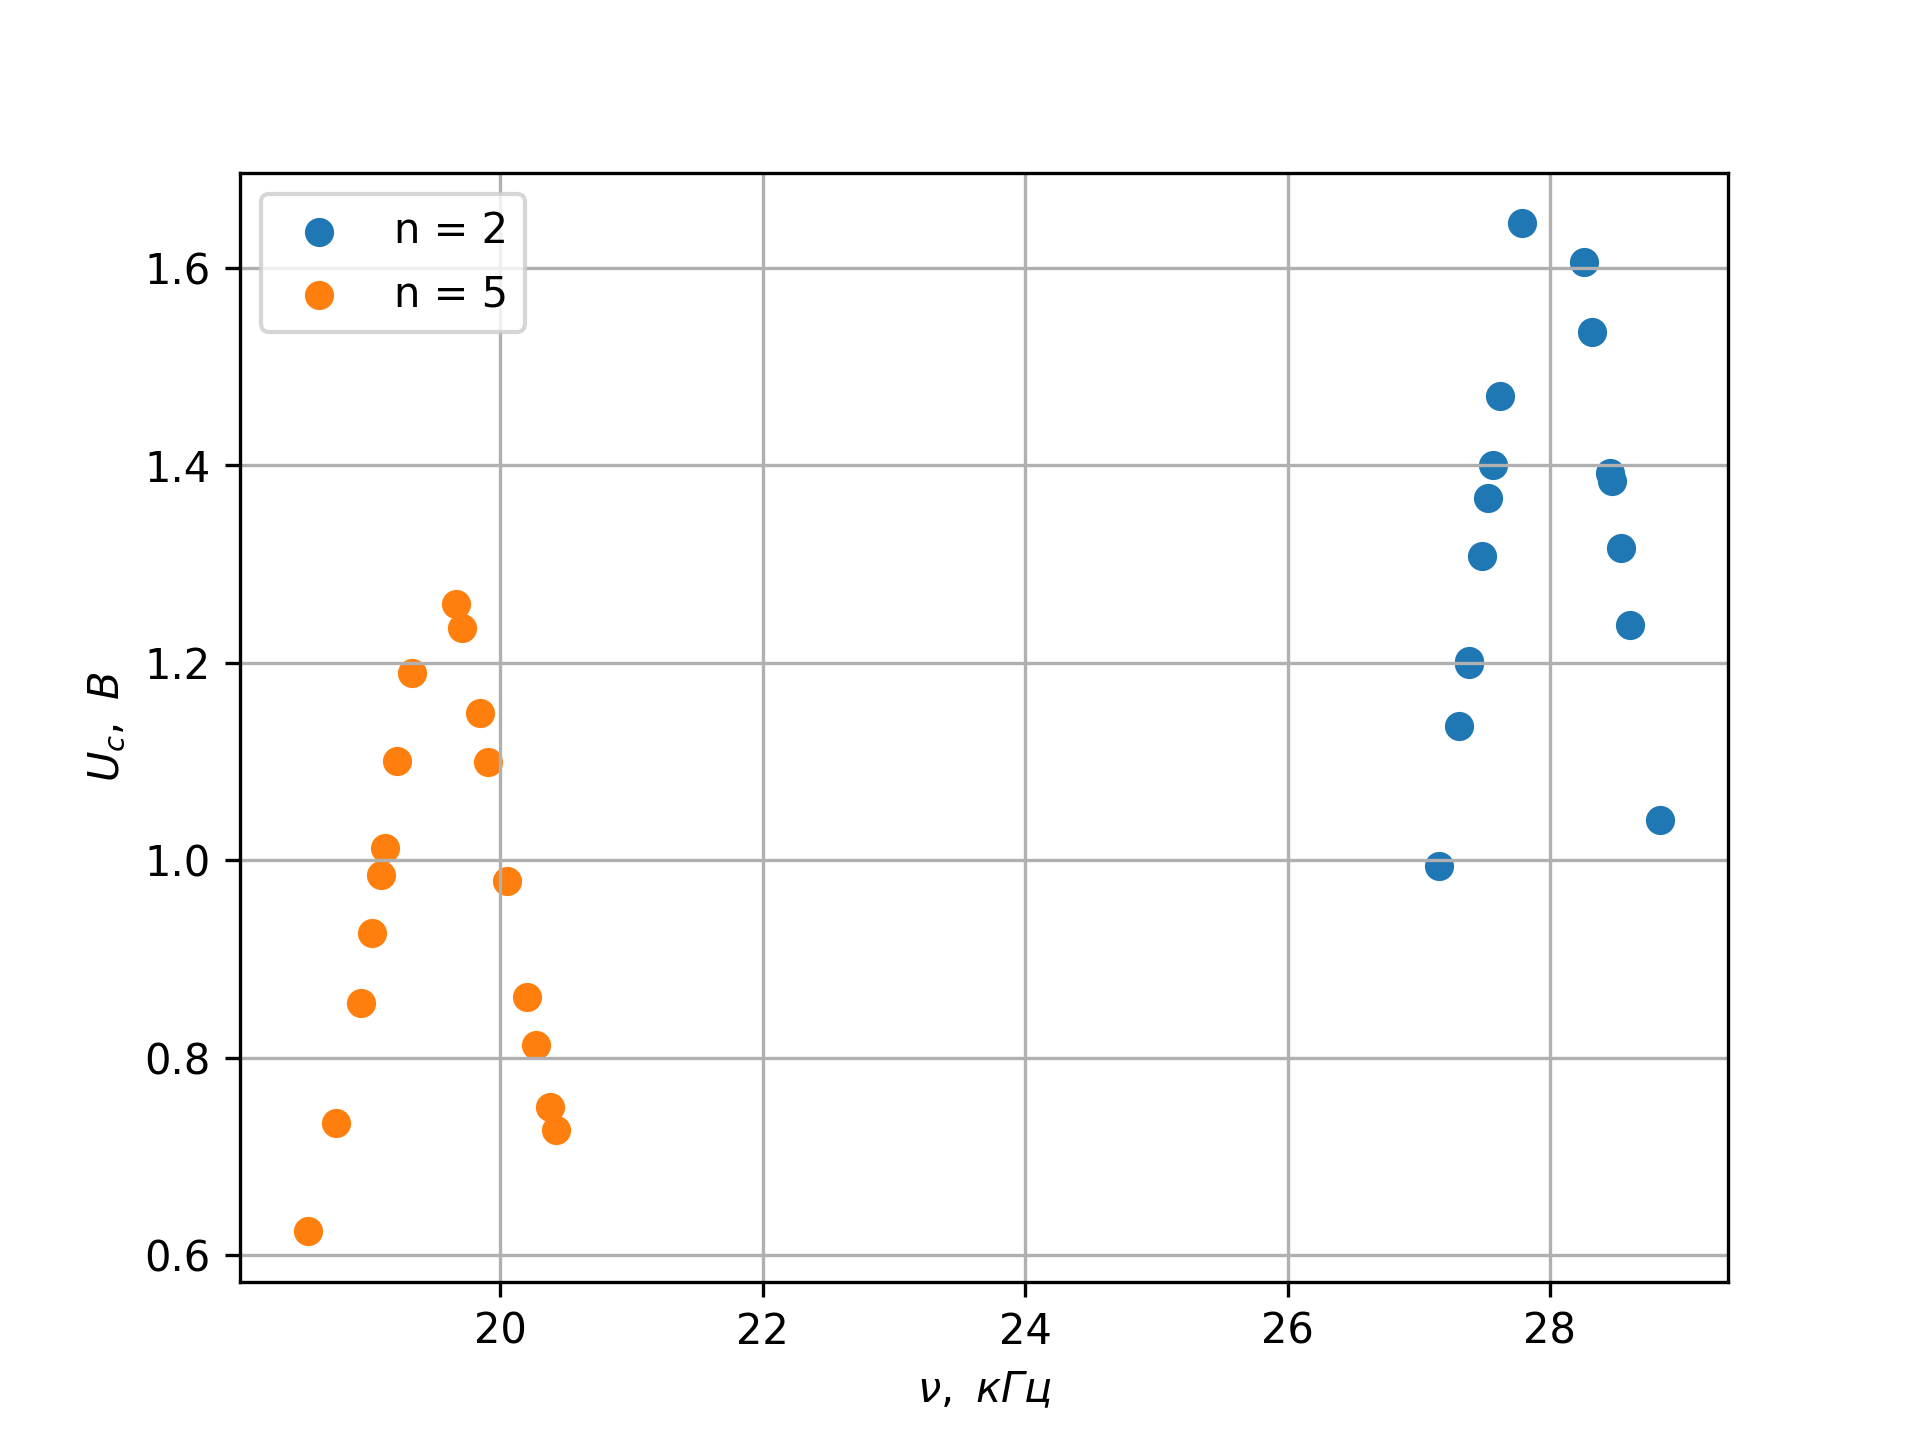
\includegraphics[scale=0.8]{images/322_1.png}
\end{figure}

АЧХ обоих контуров схожи по форме, но напряжения в контуре 2 выше чем в контуре 5.

\item Также построим на одном графике АЧХ в относительных координатах $\frac{U_C}{U_{C0}}\left(\frac{\nu}{\nu_0}\right)$.

\begin{figure}[H]
\centering
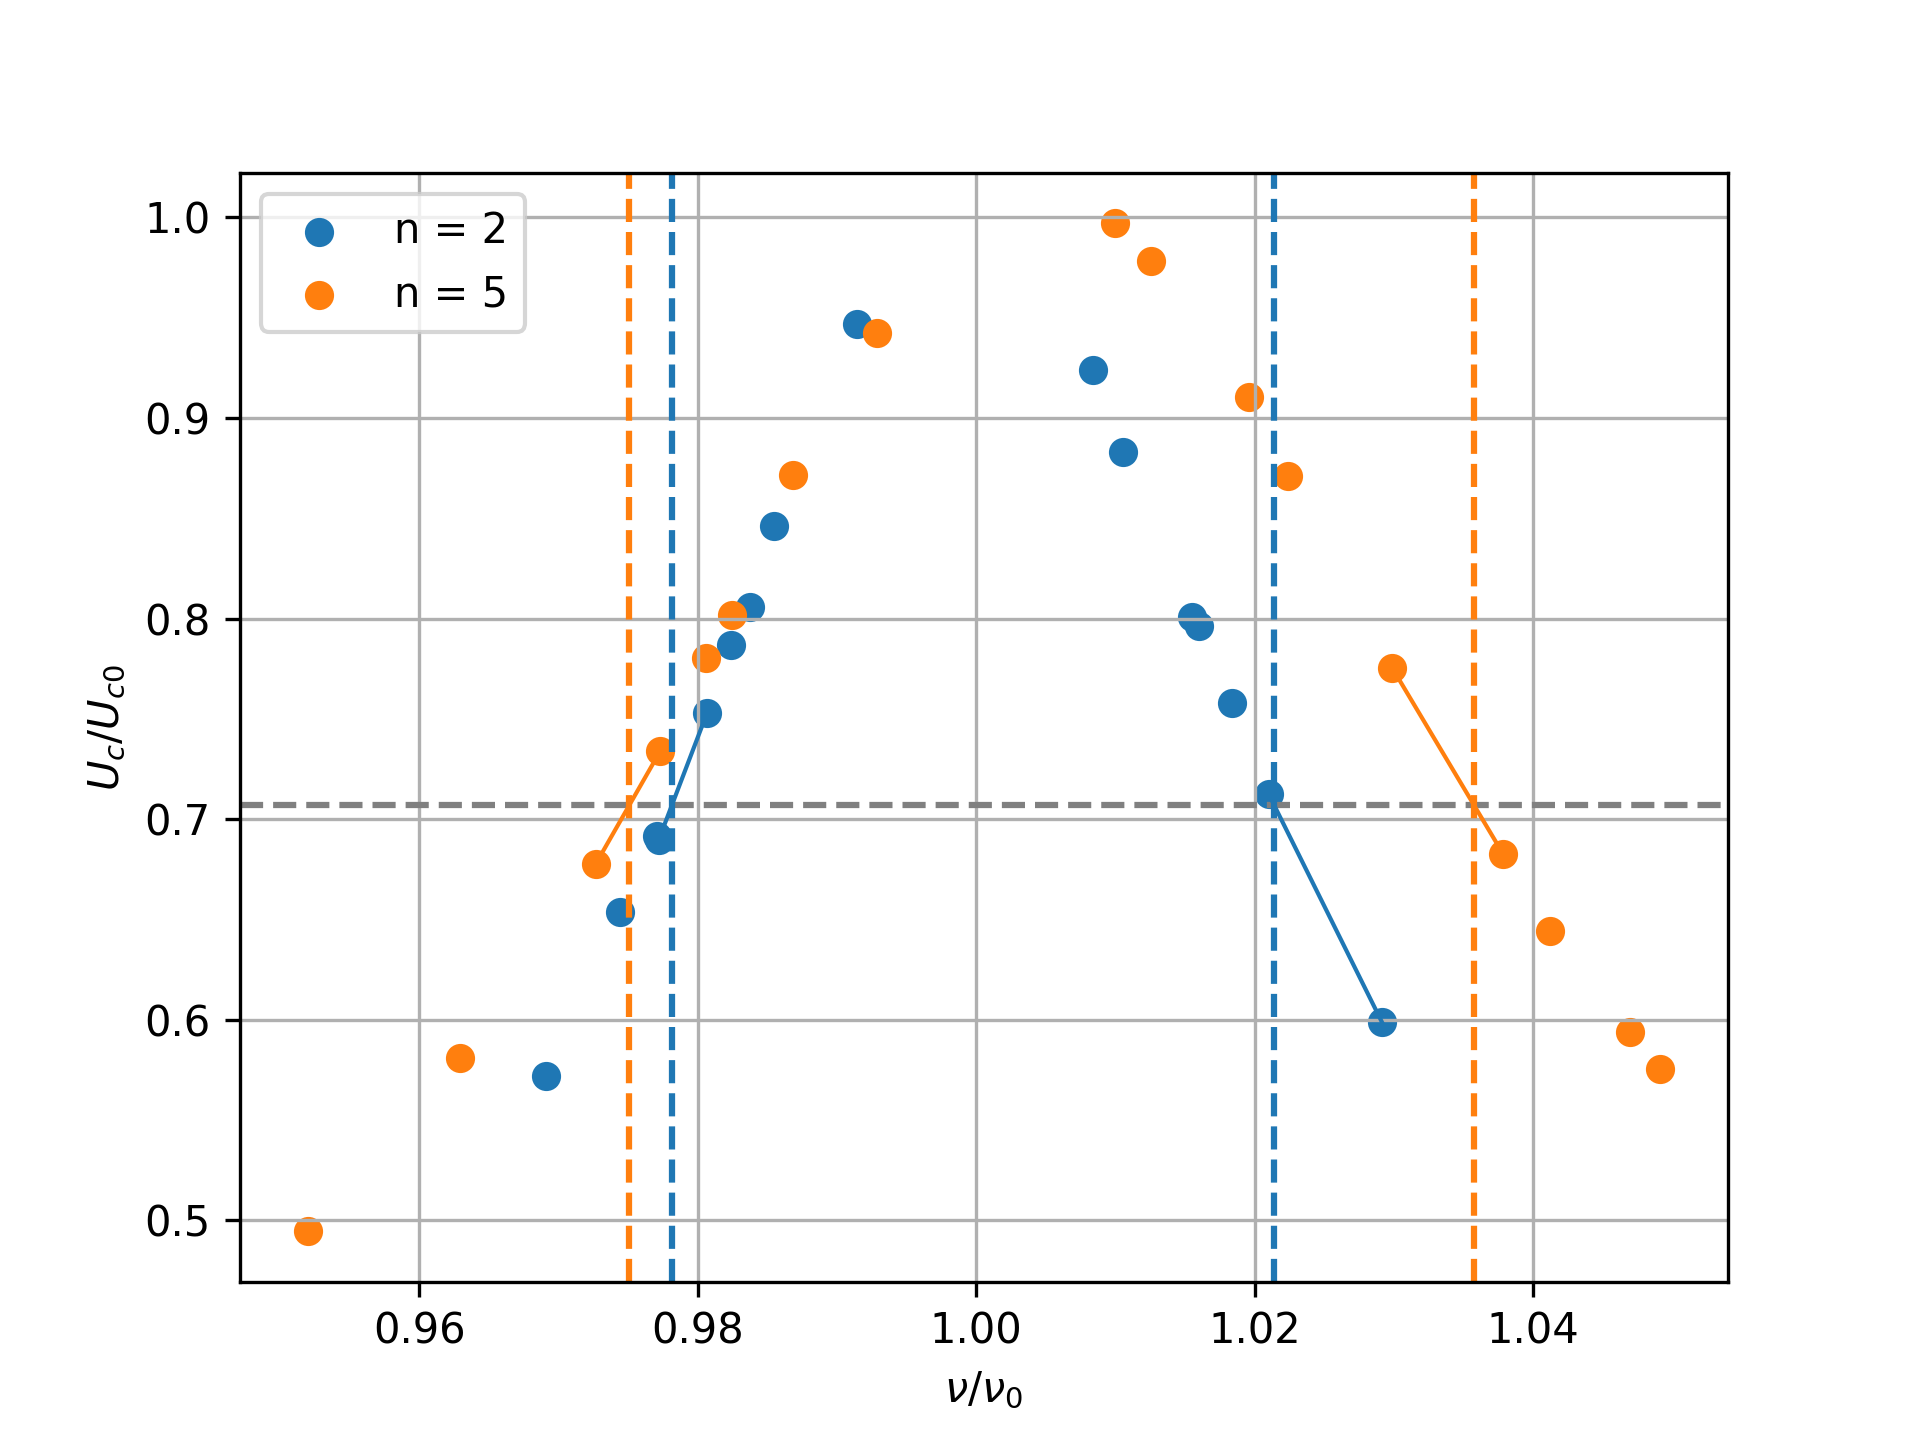
\includegraphics[scale=0.8]{images/322_2.png}
\end{figure}

По ширине резонансых кривых на уровне $\frac{1}{\sqrt{2}}$ определим добротности соответсвующих контуров.

\[Q_2=23.1\pm1.4\quad Q_5=16.5\pm1.0\]

Полученные значения очень близки к значениям из таблицы.

\item По данным измерения пункта 10 построим ФЧХ в относительных координатах $\frac{\Delta\phi}{\pi}\left(\frac{\nu}{\nu_0}\right)$.

\begin{figure}[H]
\centering
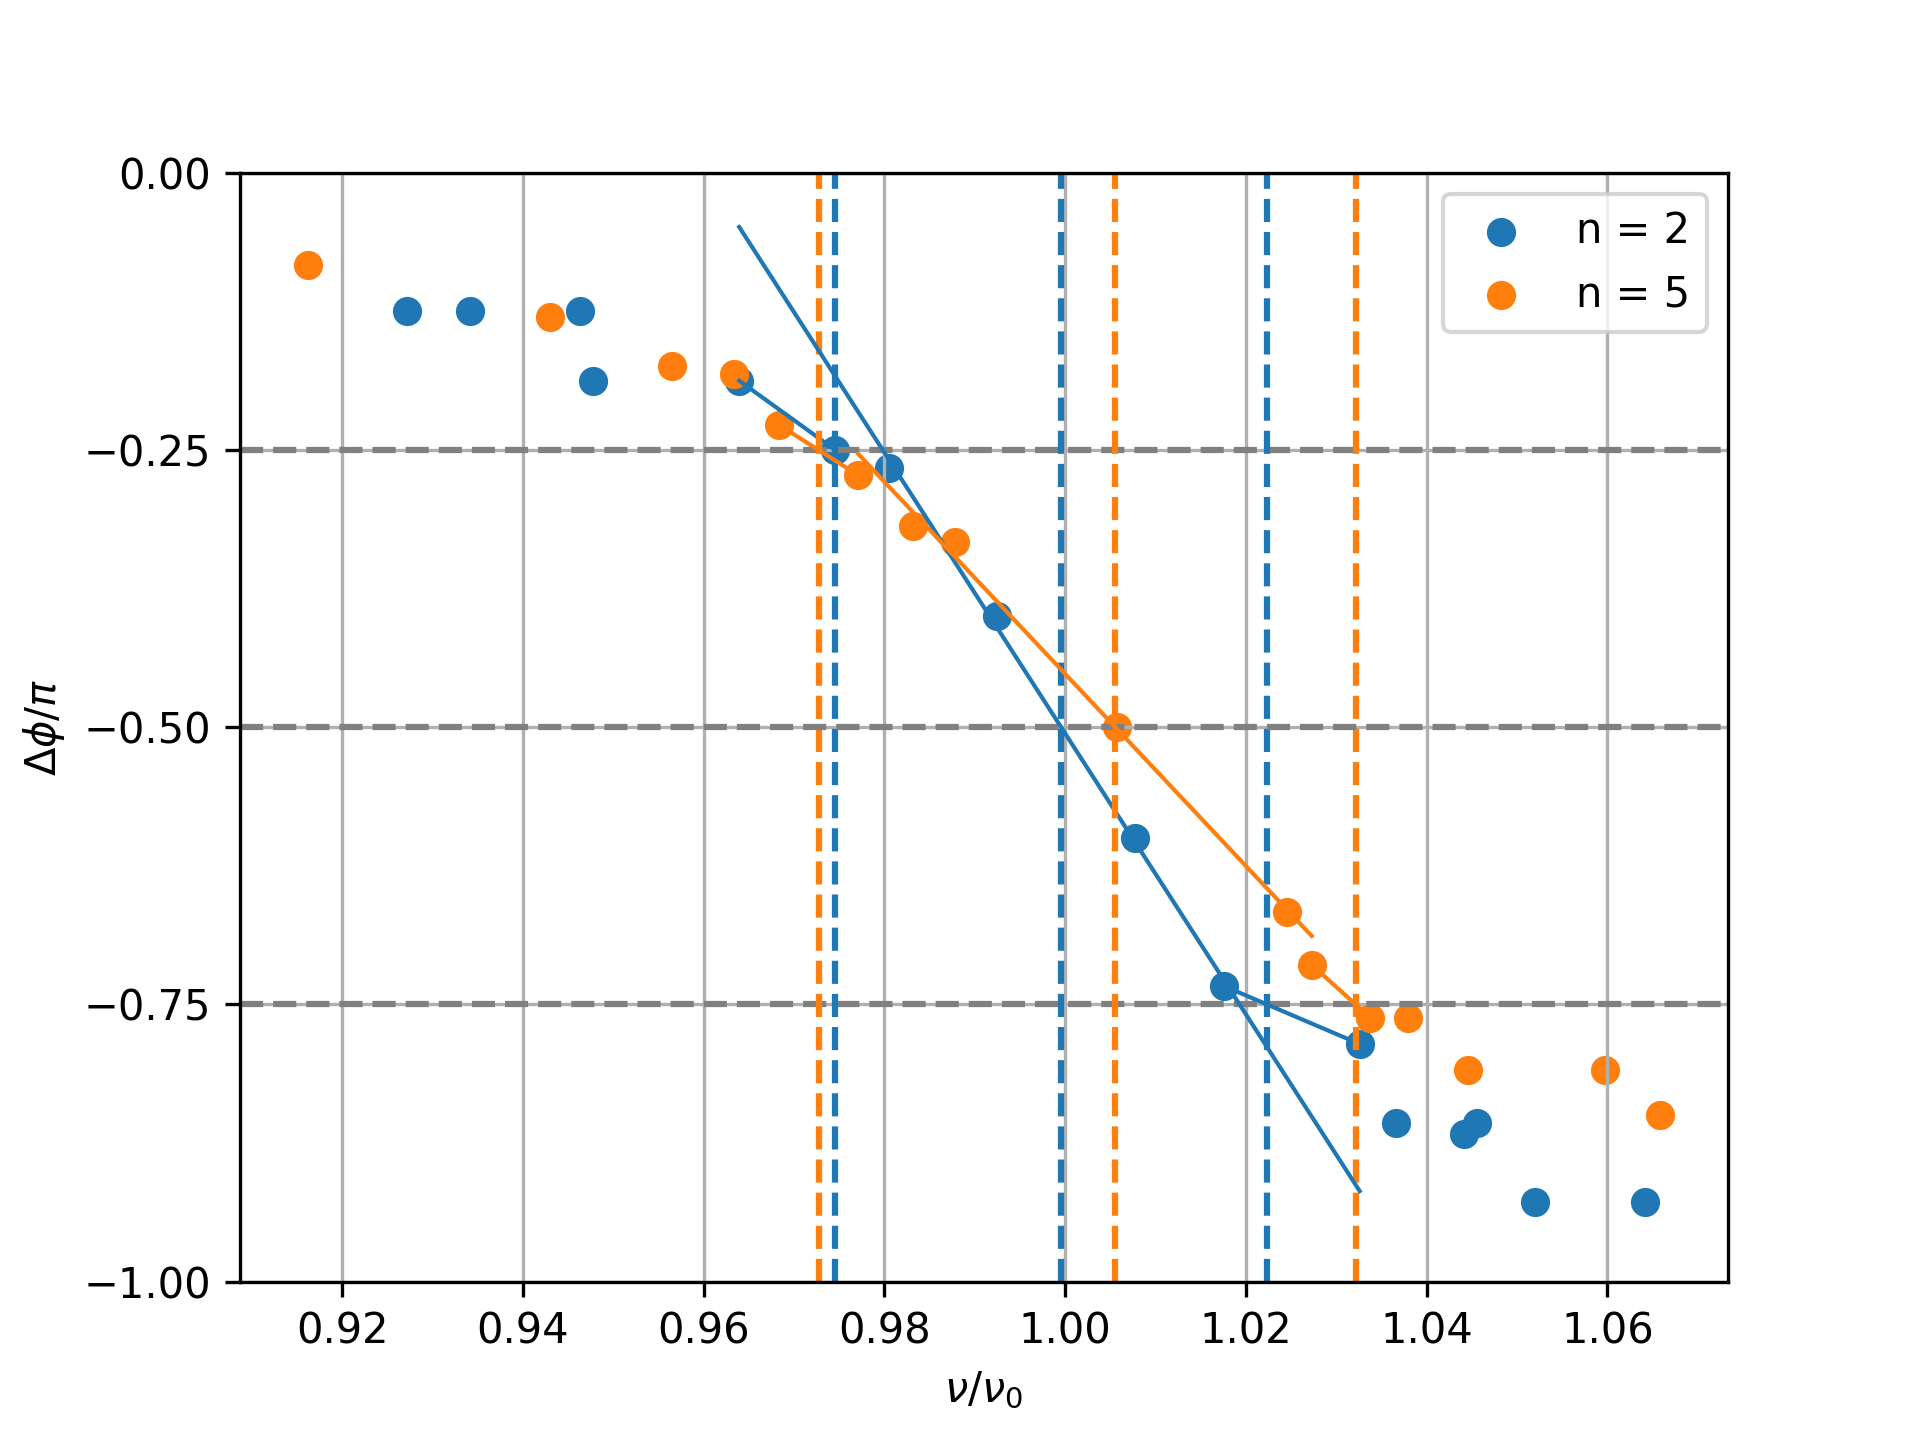
\includegraphics[scale=0.8]{images/322_3.png}
\end{figure}

По расстоянию между точками, в которых относительная разность фаз равна $-\frac{1}{4}$ и $-\frac{3}{4}$, определим добротности контуров.

\[Q_2=21\pm4\quad Q_5=17\pm3\]

Нетрудно показать, что производная ФЧХ равна $\left.\frac{d(\Delta\phi/\pi)}{d(\nu/\nu_0)}\right\vert_{\nu/\nu_0=1}=-\frac{2Q}{\pi}$. Рассчитаем добротность таким образом.

\[Q_2=19.9\pm0.6\quad Q_5=13.6\pm0.6\]

Первый способ дает более сходящиеся с предыдущими измерениями реузльтаты, несмотря на большую погрешность.

\item Построим график зависимости $R_L(f_0)$

\begin{figure}[H]
\centering
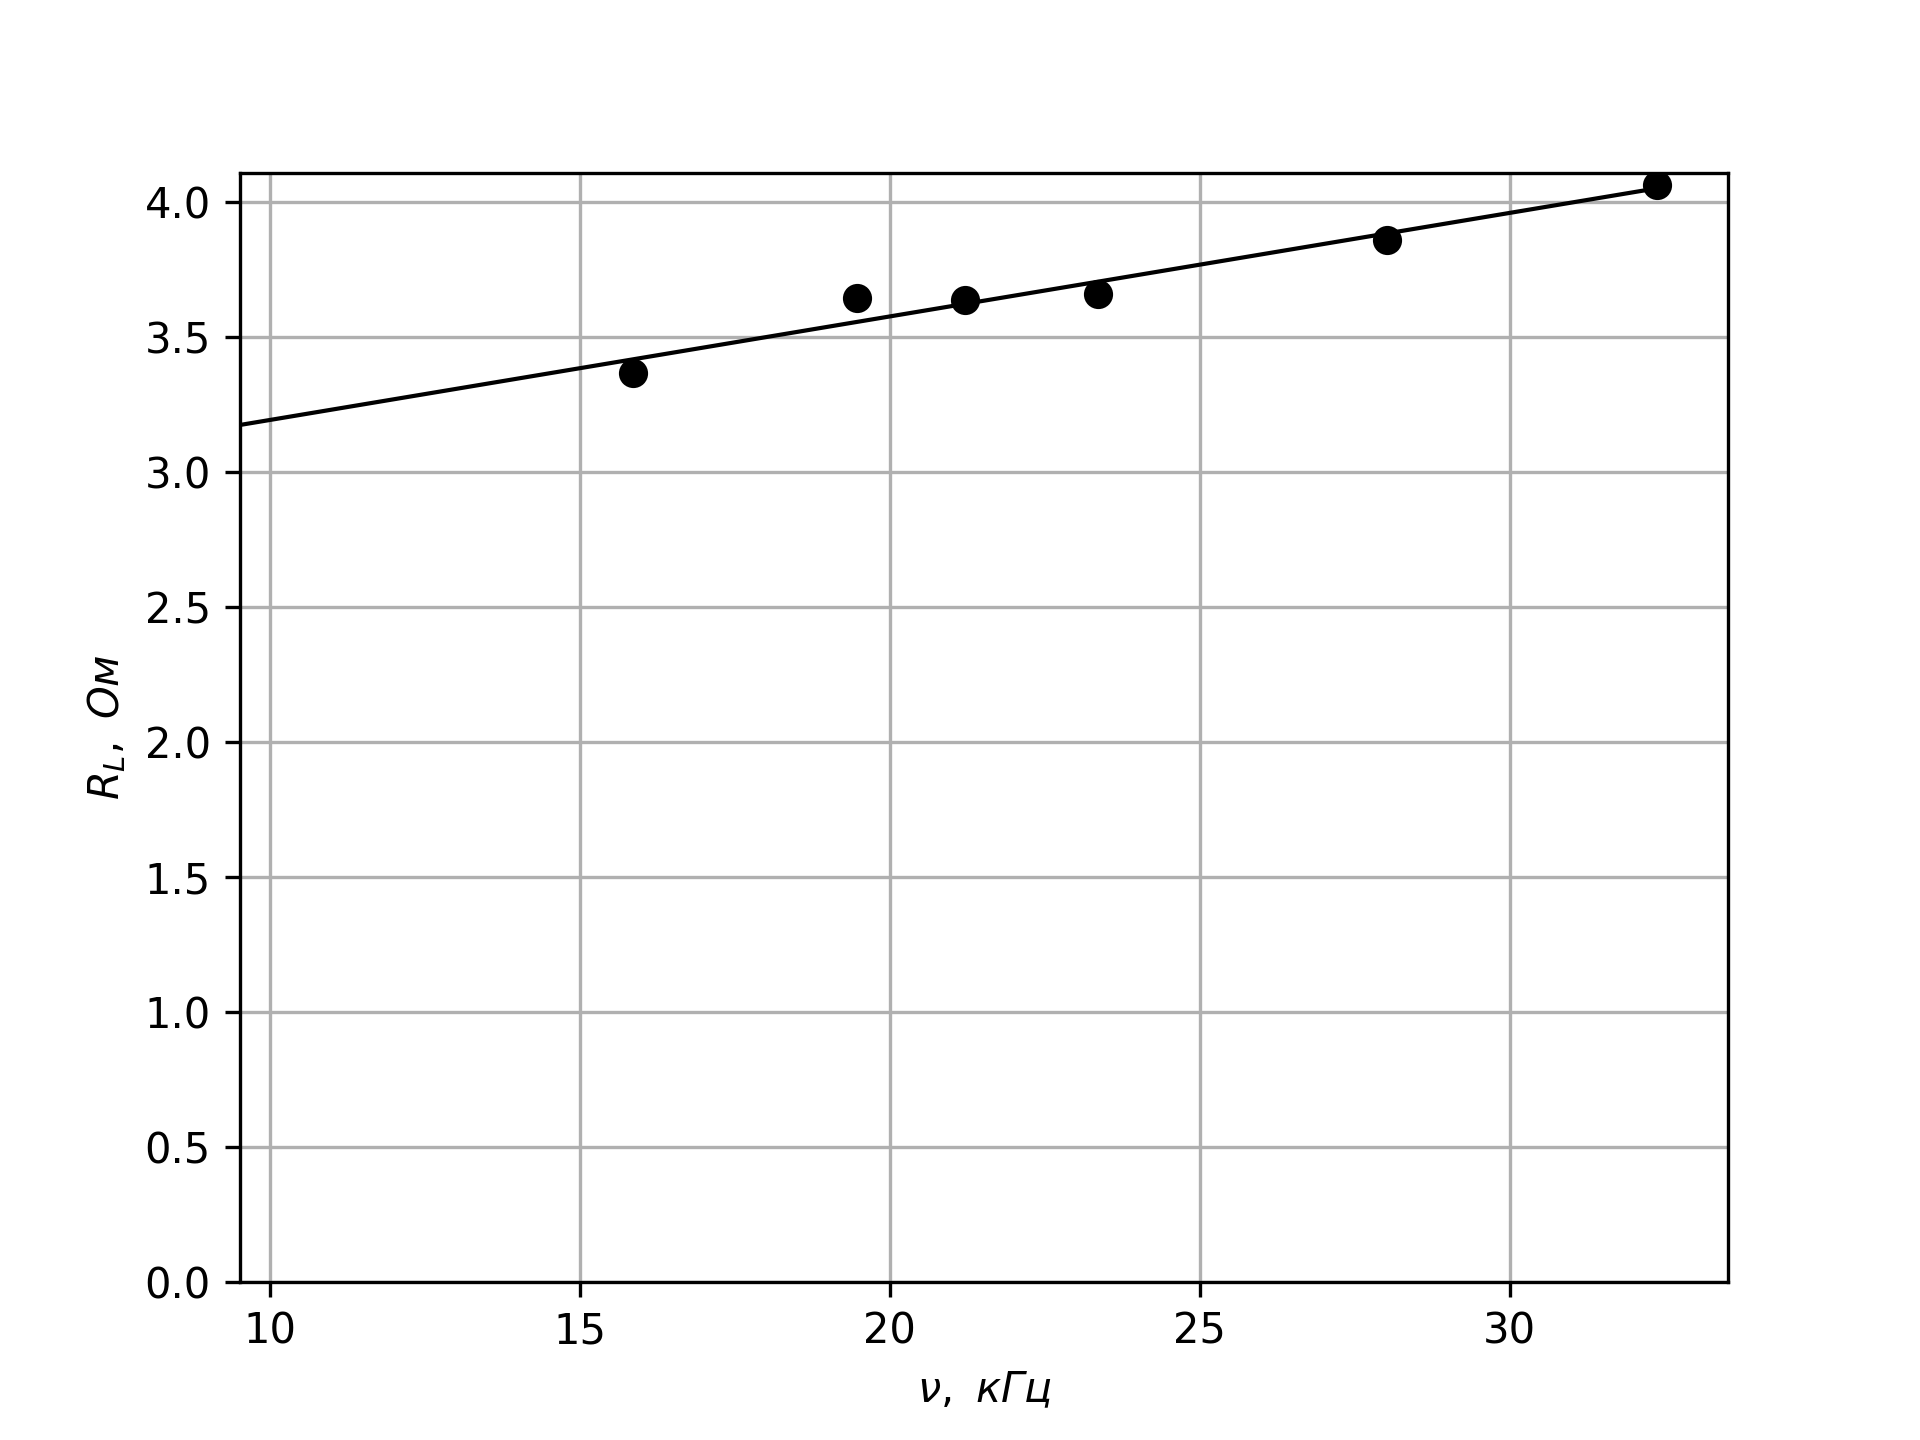
\includegraphics[scale=0.8]{images/322_4.png}
\end{figure}

\item Ниже представлена векторная диаграмма для последнего колебательного контура.

\begin{figure}[H]
\centering
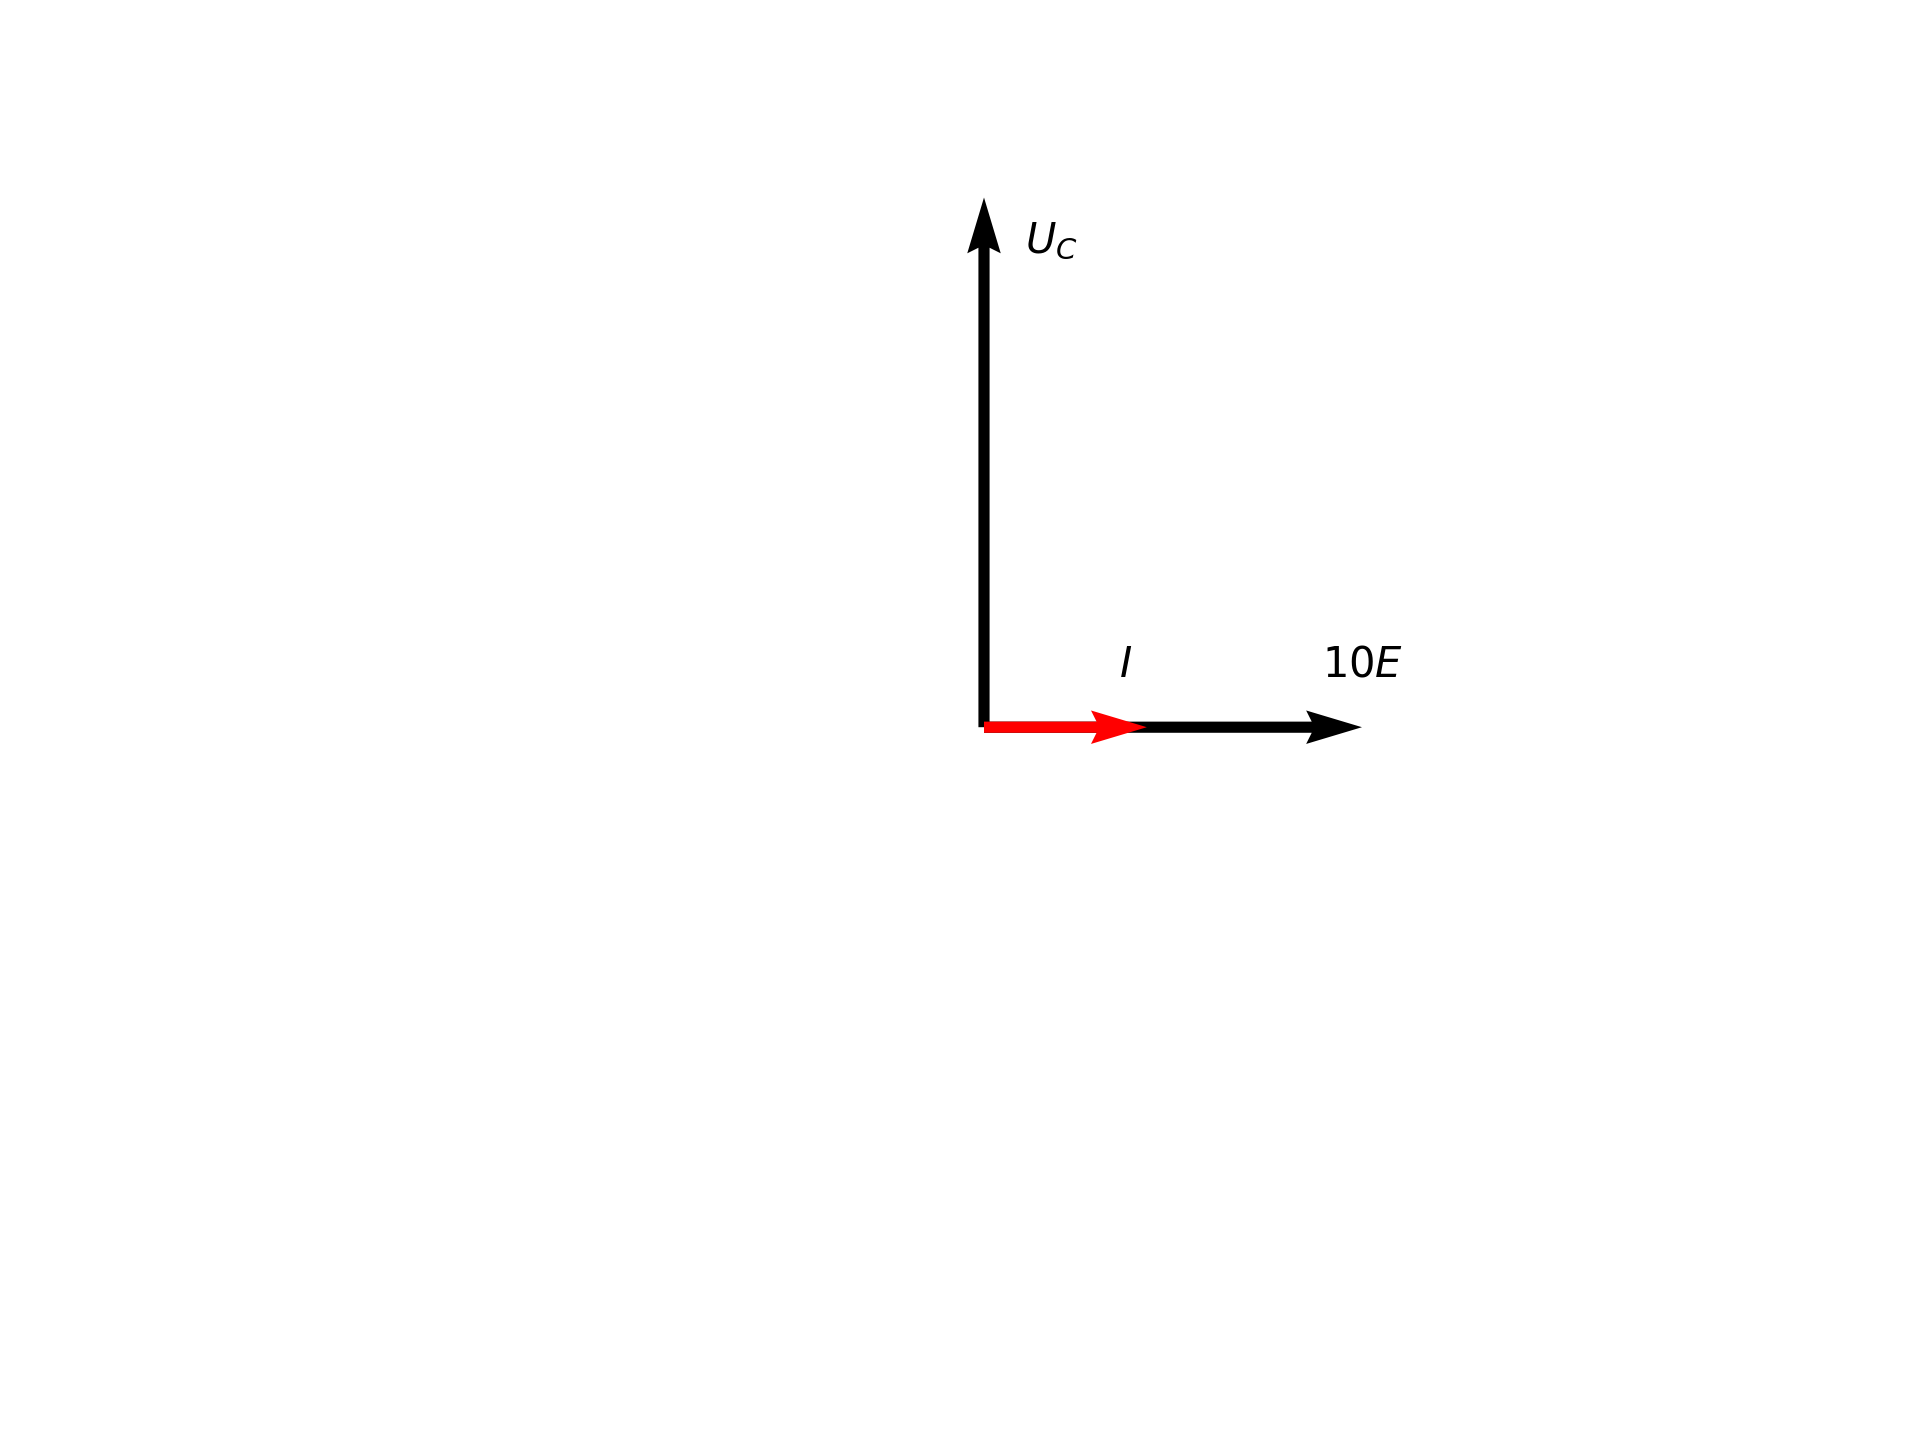
\includegraphics[scale=0.6]{images/322_5.png}
\end{figure}


\end{enumerate}

\end{document}